\documentclass[a4paper,11pt,twoside]{memoir}
\chapterstyle{veelo}


\usepackage[utf8]{inputenc}
\usepackage[T1]{fontenc}
\usepackage[english,ngerman]{babel}


\usepackage{comment} 

\usepackage{etoolbox} % fixes fatal error caused by combining bm, stackengine, hyperref (seriously?)
% http://tex.stackexchange.com/questions/22995/package-incompatibilites-etoolbox-hyperref-and-bm-standalone

\usepackage{etex} % else error on too many packages

% includes
\usepackage{algorithm}
%\usepackage{algorithmic} % conflicts with algpseudocode
\usepackage{algpseudocode}
%\newcommand*\Let[2]{\State #1 $\gets$ #2}
\algrenewcommand\alglinenumber[1]{
{\scriptsize #1}}
\algrenewcommand{\algorithmicrequire}{\textbf{Input:}}
\algrenewcommand{\algorithmicensure}{\textbf{Output:}}


%\usepackage[multiple]{footmisc} % footnotes at the same character separated by ','

\usepackage{multicol}

\usepackage{afterpage}

\usepackage{changepage} % for adjustwidth
\usepackage{caption} % for \ContinuedFloat

\usepackage{tikz}
\usetikzlibrary{shapes,arrows,backgrounds,graphs,%
matrix,patterns,arrows,decorations.pathmorphing,decorations.pathreplacing,%
positioning,fit,calc,decorations.text,shadows%
}

\usepackage{bussproofs}
\EnableBpAbbreviations


\usepackage{amsmath}
\usepackage{amsthm}
\usepackage{amssymb} % the reals
\usepackage{mathtools} % smashoperator

\usepackage{bm} % bm, bold math symbols

\usepackage{thm-restate} % restatable env

% needs extra work and fails on some label here
%\usepackage{cleveref} % cref, apparently better than autoref of hyperref 

\usepackage{nicefrac} % nicefrac

\usepackage{mathrsfs} % mathscr

\usepackage{pst-node} % http://tex.stackexchange.com/questions/35717/how-to-draw-arrows-between-parts-of-an-equation-to-show-the-math-distributive-pr

\usepackage{stackengine}

\usepackage{thmtools} % advanced thm commands (declaretheorem)


\usepackage{nameref} % reference name of thm instead of counter

\usepackage{todonotes}

% conflict with beamer
%\usepackage{paralist} % compactenum

\usepackage{hyperref}
%\hypersetup{hidelinks}  % don't give options to usepackage, it doesn't work with beamer
%\hypersetup{colorlinks=false}  % don't give options to usepackage, it doesn't work with beamer


% \usepackage{enumitem} % labels for enumerate % breaks beamer and memoir itemize


\usepackage{url} 


\usepackage[format=hang,justification=raggedright]{caption}% or e.g. [format=hang]

\usepackage{cancel} % \cancel

\usepackage{lineno}


% commands

% logic etcs
%\newcommand{\ex}[2]{\bigskip\section*{Exercise #1: \begin{minipage}[t]{.80\linewidth} \small \textnormal{\it #2} \end{minipage} } }

\newcommand{\ex}[2]{\bigskip \noindent\textbf{Exercise #1.} \textit{#2} \smallskip}

\newcommand{\comm}[1]{{\color{gray} // #1 }}


\newcommand{\true}[0]{\textbf{1}}
\newcommand{\false}[0]{\textbf{0}}
\newcommand{\tr}{\true}
\newcommand{\fa}{\false}

\newcommand{\ra}{\rightarrow}
\newcommand{\Ra}{\Rightarrow}
\newcommand{\la}{\leftarrow}
\newcommand{\La}{\Leftarrow}

\newcommand{\lra}{\leftrightarrow}
\newcommand{\Lra}{\Leftrightarrow}

\newcommand{\NKZ}{\textbf{NK2}}

%\DeclareMathOperator{\syneq}{\equiv} %spacing seems wrong, therefore defined as newcommand below
\DeclareMathOperator{\limpl}{\supset}
\DeclareMathOperator{\liff}{\lra}
\DeclareMathOperator{\semiff}{\Lra}
\newcommand{\syneq}{\equiv}
\newcommand{\union}{\cup}
\newcommand{\bigunion}{\bigcup}
\newcommand{\intersection}{\cap}
\newcommand{\bigintersection}{\bigcap}
\newcommand{\intersect}{\intersection}
\newcommand{\bigintersect}{\bigintersection}

\newcommand{\powerset}{\mathcal{P}}

\newcommand{\entails}{\vDash}
\newcommand{\notentails}{\nvDash}
\newcommand{\proves}{\vdash}

\newcommand{\vm}{\ensuremath{\vv_\mathcal{M}}}
\newcommand{\Dia}{\ensuremath{\lozenge}}

\newcommand{\spaced}[1]{\ \ #1 \ \ }
\newcommand{\spa}[1]{\spaced{#1}}
\newcommand{\spas}[1]{\;{#1}\;}
\newcommand{\spam}[1]{\;\,{#1}\;\,}

% functions
\DeclareMathOperator{\sk}{sk}
\DeclareMathOperator{\mgu}{mgu}
\DeclareMathOperator{\dom}{dom}
\DeclareMathOperator{\ran}{ran}

\DeclareMathOperator{\id}{id}
\DeclareMathOperator{\Fun}{FS}
\DeclareMathOperator{\Pred}{PS}
\DeclareMathOperator{\Lang}{L}
\DeclareMathOperator{\ar}{ar}
\DeclareMathOperator{\PI}{PI}
\DeclareMathOperator{\LI}{LI}
\DeclareMathOperator{\Congr}{Congr}
\DeclareMathOperator{\Refl}{Refl}
\DeclareMathOperator{\aiu}{au}
\DeclareMathOperator{\expa}{unfold-lift}

\newcommand{\PIinc}{\LI}
\newcommand{\PIincde}{\LIde}

\newcommand{\LIde}{\ensuremath{\LI^\Delta}}

\newcommand{\LIcl}{\ensuremath{\LI_{\operatorname{cl}}}}
\newcommand{\LIclde}{\ensuremath{\LI_{\operatorname{cl}}^\Delta}}

\newcommand{\cll}{\ensuremath{_{\operatorname{LIcl}}}}
\newcommand{\cllde}{\ensuremath{_{\operatorname{LIcl}^\Delta}}}

%\newcommand{\lifi}{\mathop{\ell\text{}i}}
\newcommand{\lifiboth}[1]{\ensuremath{\LIcl(#1)}}
\newcommand{\lifidelta}[1]{\ensuremath{\LIclde(#1)}}


%\DeclareMathOperator{\abstraction}{abstraction}

%\newcommand{\sk}{\ensuremath{\mathrm{sk}}}
%\newcommand{\mgu}{\ensuremath{\mathrm{mgu}}}
%\newcommand{\Fun}{\ensuremath{\mathrm{FS}}}
%\newcommand{\Pred}{\ensuremath{\mathrm{PS}}}
%\newcommand{\PI}{\ensuremath{\mathrm{PI}}}
%\newcommand{\Lang}{\ensuremath{\mathrm{L}}}
%\newcommand{\ar}{\ensuremath{\mathrm{ar}}}

\DeclareMathOperator{\AI}{AI}
\newcommand{\AIde}{\ensuremath{\AI^\Delta}}
\newcommand{\AImatrix}{\ensuremath{\AI_\mathrm{mat}}}
\newcommand{\AImatrixde}{\ensuremath{\AI_\mathrm{mat}^\Delta}}
\newcommand{\AImat}{\AImatrix}
\newcommand{\AImatde}{\AImatrixde}
\newcommand{\AIclause}{\ensuremath{\AI_\mathrm{cl}}}
\newcommand{\AIcl}{\AIclause}
\newcommand{\AIclde}{\AIclausede}
\newcommand{\AIclausede}{\ensuremath{\AIclause^\Delta}}
\newcommand{\fromclause}{\ensuremath{_{\operatorname{AIcl}}}}
\newcommand{\fromclausede}{\ensuremath{_{\operatorname{AIcl}^\Delta}}}
\newcommand{\cl}{\fromclause}
\newcommand{\clde}{\fromclausede}

\newcommand{\Q}{\ensuremath{Q}}

\newcommand{\AIcol}{\ensuremath{\AI_\mathrm{col}}}
\newcommand{\AIcolde}{\AIcol^\Delta}

\newcommand{\AIany}{\ensuremath{\AI_\mathrm{*}}}
\newcommand{\AIanyde}{\AIany^\Delta}

\newcommand{\AIclpre}{\AIclause^\bullet}
\newcommand{\AImatpre}{\AImatrix^\bullet}

\newcommand{\PS}{\Pred}
\newcommand{\FS}{\Fun}

\DeclareMathOperator{\LangSym}{\mathcal{L}}

%\newcommand{\mguarr}{\sim_\ra}
\newcommand{\mguarr}{\mapsto_{\mgu}}


%\newcommand{\Trans}{\ensuremath{\mathrm{T}}}
%\newcommand{\Trans}{\ensuremath{\mathrm{T}}}
\DeclareMathOperator{\Trans}{T}
\DeclareMathOperator{\TransInv}{T^{-1}}

\DeclareMathOperator{\FAX}{F_{Ax}}
\DeclareMathOperator{\EAX}{E_{Ax}}
%\newcommand{\FAX}{\ensuremath{\mathrm{F_{Ax}}}}
%\newcommand{\EAX}{\ensuremath{\mathrm{E_{Ax}}}}

%\newcommand{\TransAll}{\ensuremath{\Trans_{\mathrm{Ax}}}}
\DeclareMathOperator{\TransAll}{\Trans_{Ax}}
%\newcommand{\FAX}{\ensuremath{\mathrm{F_{Ax}}}}

\DeclareMathOperator{\defeq}{\stackrel{\mathrm{def}}{=}}

\newcommand{\subst}[1]{[#1]}
\newcommand{\abstractionOp}[1]{\{#1\}}

\newcommand{\subformdefinitional}[1]{\ensuremath{D_{\Sigma(#1)}}}


%\newcommand{\lift}[3]{\operatorname{Lift}_{#1}(#2; #3)}
%\newcommand{\lift}[3]{\operatorname{Lift}_{#1,#3}(#2)}
%\newcommand{\lift}[3]{\operatorname{Lift}_{#1,#3}[#2]}
%\newcommand{\lift}[3]{\overline{#2}_{#1,#3}}
\newcommand{\lifsym}{\ell}
%\newcommand{\lift}[3]{\lifsym_{#1,#3}[#2]}
\newcommand{\lift}[3]{\lifsym_{#1}^{#3}[#2]}
\newcommand{\liftnovar}[2]{\lifsym_{#1}[#2]}

%\newcommand{\lft}[3]{\lifsym_{#1,#2}[#3]}
\newcommand{\lft}[3]{\lift{#1}{#3}{#2}}
\newcommand{\lifboth}[1]{\lifsym[#1]}

%\newcommand{\lifi}{\mathop{\ell\text{}i}}
%\newcommand{\lifiboth}[1]{\lifi[#1]}
%\newcommand{\lifidelta}[1]{\lifi_\Delta^x[#1]}
%\newcommand{\lifideltanovar}[1]{\lifi_\Delta[#1]}

\newcommand{\lifdelta}[1]{\lift{\Delta}{#1}{x}}
\newcommand{\lifdeltanovar}[1]{\liftnovar{\Delta}{#1}}
\newcommand{\lifgamma}[1]{\lift{\Gamma}{#1}{y}}
\newcommand{\lifgammanovar}[1]{\liftnovar{\Gamma}{#1}}
\newcommand{\lifphinovar}[1]{\liftnovar{\Phi}{#1}}
\newcommand{\lifphi}[1]{\lift{\Phi}{#1}{z}}

\DeclareMathOperator{\arr}{\mathcal{A}}
%\DeclareMathOperator{\arrFinal}{{\mathcal{A}^{\bm*}}}
\DeclareMathOperator{\arrFinal}{{\mathcal{\bm{\hat}A}}}
\DeclareMathOperator{\warr}{\marr}
\DeclareMathOperator{\marr}{\mathcal{M}}

\DeclareMathOperator{\apath}{\leadsto}
\DeclareMathOperator{\mpath}{\leadsto_=}
\DeclareMathOperator{\notapath}{\not\leadsto}
\DeclareMathOperator{\notmpath}{\not\leadsto_=}

\newcommand{\ltArrC}{<_{\arrFinal(C)}}
\newcommand{\ltAC}{<_{\arr(C)}}
\newcommand{\ltArrCOne}{<_{\arrFinal(C_1)}}
\newcommand{\ltArrCTwo}{<_{\arrFinal(C_2)}}
%\newcommand{\ltArrC}{<_{\scalebox{0.6}{$\arrFinal(C)$}}}
\newcommand{\ltArr}{<_{\scalebox{0.6}{$\arrFinal$}}}

\newcommand{\bhat}{\bm\hat}
\newcommand{\bbar}{\bm\bar}
\newcommand{\bdot}{\bm\dot}

%\usepackage{yfonts}
\usepackage{upgreek}
\DeclareMathAlphabet{\mathpzc}{OT1}{pzc}{m}{it}
%\DeclareMathOperator{\pos}{\mathscr{P}}
%\DeclareMathOperator{\pos}{\mathpzc{p}}
%\DeclareMathOperator{\pos}{{\rho}}
\DeclareMathOperator{\pos}{{\operatorname P}}
%\DeclareMathOperator{\pos}{P}
\DeclareMathOperator{\poslit}{\pos_\mathrm{lit}}
\DeclareMathOperator{\posterm}{\pos_\mathrm{term}}
%\newcommand{\poslit}[1]{\ensuremath{p_\text{lit}(#1)}}
%\newcommand{\posterm}[1]{\ensuremath{p_\text{term}(#1)}}
\newcommand{\at}[1]{|_{#1}}

\newcommand{\UICm}[1]{\UnaryInfCm{#1}}
\newcommand{\UnaryInfCm}[1]{\UnaryInfC{$#1$}}
\newcommand{\BICm}[1]{\BinaryInfCm{#1}}
\newcommand{\BinaryInfCm}[1]{\BinaryInfC{$#1$}}
\newcommand{\RightLabelm}[1]{\RightLabel{$#1$}}
\newcommand{\LeftLabelm}[1]{\LeftLabel{$#1$}}
\newcommand{\AXCm}[1]{\AxiomCm{#1}}
\newcommand{\AxiomCm}[1]{\AxiomC{$#1$}}
\newcommand{\mt}[1]{\textnormal{#1}}

\newcommand{\UnaryInfm}[1]{\UnaryInf$#1$}
\newcommand{\BinaryInfm}[1]{\BinaryInf$#1$}
\newcommand{\Axiomm}[1]{\Axiom$#1$}



% math
\newcommand{\calI}{\ensuremath{\mathcal{I}}}

\newcommand{\tupleShort}[2]{\ensuremath{(#1_1,\dotsc,#1_{#2})}}
\newcommand{\tuple}[2]{\ensuremath{(#1_1,\:#1_2\:,\dotsc,\:#1_{#2})}}
\newcommand{\setelements}[2]{\ensuremath{\{#1_1,\:#1_2\:,\dotsc,\:#1_{#2}\}}}
\newcommand{\pathelements}[2]{\ensuremath{ (#1_1,\:#1_2\:,\dotsc,\:#1_{#2}) }}

\newcommand{\elems}[1]{\ensuremath{#1_1,\dotsc, #1_{n}) }}

\newcommand{\defiemph}[1]{\emph{#1}}

\newcommand{\setofbases}{\ensuremath{\mathcal{B}}}
\newcommand{\setofcircuits}{\ensuremath{\mathcal{C}}}

\newcommand{\reals}{\ensuremath{\mathbb{R}}}
\newcommand{\integers}{\ensuremath{\mathbb{Z}}} 
\newcommand{\naturalnumbers}{\ensuremath{\mathbb{N}}}

% general
\newcommand{\zit}[3]{#1\ \cite{#2}, #3}
\newcommand{\zitx}[2]{#1\ \cite{#2}}
\newcommand{\footzit}[3]{\footnote{\zit{#1}{#2}{#3}}}
\newcommand{\footzitx}[2]{\footnote{\zitx{#1}{#2}}}

\newcommand{\ite}{\begin{itemize}}
\newcommand{\ete}{\end{itemize}}

\newcommand{\bfr}{\begin{frame}}
\newcommand{\efr}{\end{frame}}

\newcommand{\ilc}[1]{\texttt{#1}}


% misc

% multiframe
\usepackage{xifthen}% provides \isempty test
% new counter to now which frame it is within the sequence
\newcounter{multiframecounter}
% initialize buffer for previously used frame title
\gdef\lastframetitle{\textit{undefined}}
% new environment for a multi-frame
\newenvironment{multiframe}[1][]{%
\ifthenelse{\isempty{#1}}{%
% if no frame title was set via optional parameter,
% only increase sequence counter by 1
\addtocounter{multiframecounter}{1}%
}{%
% new frame title has been provided, thus
% reset sequence counter to 1 and buffer frame title for later use
\setcounter{multiframecounter}{1}%
\gdef\lastframetitle{#1}%
}%
% start conventional frame environment and
% automatically set frame title followed by sequence counter
\begin{frame}%
\frametitle{\lastframetitle~{\normalfont \Roman{multiframecounter}}}%
}{%
\end{frame}%
}




% http://texfragen.de/hurenkinder_und_schusterjungen
\usepackage[all]{nowidow}



% force no overlong lines:
%\tolerance=1 % tolerance for how badly spaced lines are allowed, less means "better" lines
\tolerance=500 %  need more tolerance for equations
%\emergencystretch=\maxdimen
%\emergencystretch=200pt
%\setlength{\emergencystretch}{3em}
%\hyphenpenalty=10000 % forces no hyphenation
%\hbadness=10000


% http://tex.stackexchange.com/questions/35717/how-to-draw-arrows-between-parts-of-an-equation-to-show-the-math-distributive-pr
\tikzset{square arrow/.style={to path={ -- ++(.0,-.15)  -| (\tikztotarget)}}}
\tikzset{square arrow2/.style={to path={ -- ++(.0,-.25)  -| (\tikztotarget)}}}
%\tikzset{square arrow/.style={to path={ -- ++(00,-.01) -- ++(0.5,-0.1) -- ++(0.5,-0.1) -| (\tikztotarget)},color=red}}


% have arrows from a to b and from c to d here
% just use: texttext\arrowA texttest \arrowB texttext
\newcommand{\arrowA}{\tikz[overlay,remember picture] \node (a) {};}
\newcommand{\arrowB}{\tikz[overlay,remember picture] \node (b) {};}
\newcommand{\drawAB}{
	\tikz[overlay,remember picture]
	{\draw[->,bend left=5,color=red] (a.south) to (b.south);}
	%{\draw[->,square arrow,color=red] (a.south) to (b.south);}
}
\newcommand{\arrowAP}{\tikz[overlay,remember picture] \node (ap) {};}
\newcommand{\arrowBP}{\tikz[overlay,remember picture] \node (bp) {};}
\newcommand{\drawABP}{
	\tikz[overlay,remember picture]
	{\draw[->,bend right=5,color=red] (ap.south) to (bp.south);}
	%{\draw[->,square arrow,color=red] (a.south) to (b.south);}
}

\newcommand{\arrowAB}{\tikz[overlay,remember picture] \node (ab) {};}
\newcommand{\arrowBA}{\tikz[overlay,remember picture] \node (ba) {};}
\newcommand{\drawAABB}{
	\tikz[overlay,remember picture]
	%{\draw[->,bend left=80] (a.north) to (b.north);}
	{\draw[->,square arrow,color=brown] (ab.south) to (ba.south);
	\draw[->,square arrow,color=brown] (ba.south) to (ab.south);}
}


\newcommand{\arrowCD}{\tikz[overlay,remember picture] \node (cd) {};}
\newcommand{\arrowDC}{\tikz[overlay,remember picture] \node (dc) {};}
\newcommand{\drawCCDD}{
	\tikz[overlay,remember picture]
	%{\draw[->,bend left=80] (a.north) to (b.north);}
	{\draw[<->,dashed,square arrow,color=green] (cd.south) to (dc.south); }
}



\newcommand{\arrowC}{\tikz[overlay,remember picture] \node (c) {};}
\newcommand{\arrowD}{\tikz[overlay,remember picture] \node (d) {};}
\newcommand{\drawCD}{
	\tikz[overlay,remember picture]
	{\draw[->,square arrow,color=blue] (c.south) to (d.south);}
}

\newcommand{\arrowE}{\tikz[overlay,remember picture] \node (e) {};}
\newcommand{\arrowF}{\tikz[overlay,remember picture] \node (f) {};}
\newcommand{\drawEF}{
	\tikz[overlay,remember picture]
	{\draw[->,square arrow2,color=orange] (e.south) to (f.south);}
}


\newcommand{\arrAP}{\arrowAP}
\newcommand{\arrBP}{\arrowBP}
\newcommand{\arrA}{\arrowA}
\newcommand{\arrB}{\arrowB}
\newcommand{\arrC}{\arrowC}
\newcommand{\arrD}{\arrowD}
\newcommand{\arrE}{\arrowE}
\newcommand{\arrF}{\arrowF}


\DeclareMathOperator{\simgeq}{\scalebox{0.92}{$\gtrsim$}}

\newcommand{\refsub}[2]{\hyperref[#2]{\ref*{#1}.\ref*{#2}}}

%\newcommand{\sigmarange}[2]{\sigma_{#1}^{#2} }
\newcommand{\sigmarange}[2]{\sigma_{(#1,#2)} }
\newcommand{\sigmaz}[1]{\sigmarange{0}{#1} }
\newcommand{\sigmazi}[0]{\sigmaz{i} }

\DeclareMathOperator{\lit}{lit}

%\def\fCenter{\ \proves\ }
\def\fCenter{\proves}

\newcommand{\prflbl}[2]{\RightLabel{\footnotesize $#1, #2$} }
%\newcommand{\prflblid}[1]{\RightLabel{$#1, \id$} }
\newcommand{\prflblid}[1]{\RightLabel{\footnotesize $#1$} }

\DeclareMathOperator{\resruleres}{res}
\DeclareMathOperator{\resrulefac}{fac}
\DeclareMathOperator{\resrulepar}{par}
\newcommand{\lkrule}[2]{\ensuremath{\operatorname{#1}:#2}} % operatorname fixes spacing issues for =

\newcommand{\parti}[4]{\ensuremath{ \langle (#1; #2), (#3; #4)\rangle  }}

\newcommand{\partisym}{\ensuremath{\chi}}

\newcommand{\occur}[1]{\ensuremath{[#1]}}
\newcommand{\occ}[1]{\occur{#1}}

\newcommand{\occurat}[2]{\ensuremath{{\occur{#1}_{#2}}}}
\newcommand{\occat}[2]{\occurat{#1}{#2}}
\newcommand{\occatp}[1]{\occurat{#1}{p}}
\newcommand{\occatq}[1]{\occurat{#1}{q}}

\newcommand{\colterm}[1]{\zeta_{#1}}



% fix restateable spacing 
%http://tex.stackexchange.com/questions/111639/extra-spacing-around-restatable-theorems

\makeatletter

\def\thmt@rst@storecounters#1{%
%THIS IS THE LINE I ADDED:
\vspace{-1.9ex}%
  \bgroup
        % ugly hack: save chapter,..subsection numbers
        % for equation numbers.
  %\refstepcounter{thmt@dummyctr}% why is this here?
  %% temporarily disabled, broke autorefname.
  \def\@currentlabel{}%
  \@for\thmt@ctr:=\thmt@innercounters\do{%
    \thmt@sanitizethe{\thmt@ctr}%
    \protected@edef\@currentlabel{%
      \@currentlabel
      \protect\def\@xa\protect\csname the\thmt@ctr\endcsname{%
        \csname the\thmt@ctr\endcsname}%
      \ifcsname theH\thmt@ctr\endcsname
        \protect\def\@xa\protect\csname theH\thmt@ctr\endcsname{%
          (restate \protect\theHthmt@dummyctr)\csname theH\thmt@ctr\endcsname}%
      \fi
      \protect\setcounter{\thmt@ctr}{\number\csname c@\thmt@ctr\endcsname}%
    }%
  }%
  \label{thmt@@#1@data}%
  \egroup
}%

\makeatother




\newcommand{\mymark}[1]{\ensuremath{(#1)}}
\newcommand{\markA}{\mymark \circ}
\newcommand{\markB}{\mymark *}
\newcommand{\markC}{\mymark \divideontimes}

\newcommand{\wrong}[1]{{\color{red}WRONG: #1}}
\newcommand{\NB}[1]{{\color{blue}NB: #1}}
\newcommand{\hl}[1]{{\color{orange} #1}}
\newcommand{\mytodo}[1]{{\color{red}TODO: #1}}
\newcommand{\largered}[1]{{

	  \LARGE\bfseries\color{red}
		#1

}}
\newcommand{\largeblue}[1]{{

	  \large\bfseries\color{blue}
		#1

}}




\usepackage{ulem} %  \dotuline{dotty} \dashuline{dashing} \sout{strikethrough}
\normalem

\usepackage{tabu} % tabular also in math mode (and much more)

\usepackage[color]{changebar} %  \cbstart, \cbend
\cbcolor{red}



% http://tex.stackexchange.com/questions/7032/good-way-to-make-textcircled-numbers
\newcommand*\circled[1]{\tikz[baseline=(char.base)]{
\node[shape=circle,draw,inner sep=2pt] (char) {#1};}}



% http://tex.stackexchange.com/questions/43346/how-do-i-get-sub-numbering-for-theorems-theorem-1-a-theorem-1-b-theorem-2

\makeatletter
\newenvironment{subtheorem}[1]{%
  \def\subtheoremcounter{#1}%
  \refstepcounter{#1}%
  \protected@edef\theparentnumber{\csname the#1\endcsname}%
  \setcounter{parentnumber}{\value{#1}}%
  \setcounter{#1}{0}%
  \expandafter\def\csname the#1\endcsname{\theparentnumber.\Alph{#1}}%
  \ignorespaces
}{%
  \setcounter{\subtheoremcounter}{\value{parentnumber}}%
  \ignorespacesafterend
}
\makeatother
\newcounter{parentnumber}


\usepackage{tabularx}% http://ctan.org/pkg/tabularx
\newcolumntype{Y}{>{\centering\arraybackslash}X}

\newcommand{\mycols}[2][3]{
	\noindent\begin{tabularx}{\textwidth}{*{#1}{Y}}
		#2
	\end{tabularx}%
}


\newcommand{\definethms}{

	%\declaretheorem[title=Theorem,qed=$\triangle$,parent=chapter]{thm}
	\newcommand{\thmqed}{$\square$} % for thms without proof
	\newcommand{\propqed}{$\square$} % for props without proof
	\declaretheorem[title=Theorem]{thm}
	\declaretheorem[title=Proposition,sibling=thm]{prop}
	\declaretheorem[title=Conjectured Proposition,sibling=thm]{cprop}

	%\declaretheorem[title=Lemma,parent=chapter]{lemma}
	\declaretheorem[sibling=thm]{lemma}
	\declaretheorem[sibling=thm,title=Conjectured Lemma]{clemma}
	\declaretheorem[title=Corollary,sibling=thm]{corr}
	\declaretheorem[sibling=thm,title=Definition,style=definition,qed=$\triangle$]{defi}
	%\declaretheorem[title=Definition,qed=$\triangle$,parent=chapter]{defi}
	\declaretheorem[title=Example,style=definition,qed=$\triangle$,sibling=thm]{exa}

	\declaretheorem[sibling=thm,title=Conjecture]{conj}

	\declaretheorem[title=Remark,style=remark,numbered=no,qed=$\triangle$]{remark}


}

\usepackage[matha]{mathabx} % the locial operators here have more space around them and [ and ] are thicker, also langle and rangle are a bit nicer; subseteq looks a bit weird

%\usepackage{MnSymbol} % again other symbols


\newcommand{\inference}{\ensuremath{\iota}}

\usepackage{cases} % numcases


\usepackage{TUINFDA}

\usepackage{url}
\usepackage{hyperref}					% links in pdf
\usepackage{graphicx}            			% Figures
\usepackage{verbatim}            			% Code-Environment
%\usepackage[lined,linesnumbered,algochapter]{algorithm2e} % Algorithm-Environment

\usepackage{pgf}					
\usepackage{tikz}					% tikz graphics
\usetikzlibrary{arrows,automata}

%\usepackage{bibgerm,cite}       % Deutsche Bezeichnungen, Automatisches Zusammenfassen von Literaturstellen

%\usepackage[ngerman]{varioref}  % Querverweise
% to use the german charset include cp850 for MS-DOS, ansinew for Windows and latin1 for Linux.
% \usepackage[latin1]{inputenc}

\thesistitle{Title of the Thesis}
\thesissubtitle{Optional Subtitle} % optional
\thesisdate{TT.MM.JJJJ}

% all titles and designations have to be gender-related!
\thesisdegree{Diplom-Ingenieur}{Diplom-Ingenieur}
\thesiscurriculum{Computational Intelligence}{Computational Intelligence} % your study
\thesisverfassung{Verfasser} % Verfasser
\thesisauthor{Bernhard Mallinger} % your name
\thesisauthoraddress{Gassergasse 25/17-18, 1050 Wien} % your address
\thesismatrikelno{0707663} % your registration number

\thesisbetreins{Ass.Prof.~Stefan Hetzl}
\thesisbetrzwei{Dr. Vorname Familienname}
\thesisbetrdrei{Dr. Vorname Familienname} % optional

% define page numbering styles
\makepagestyle{numberCorner}
\makeevenfoot{numberCorner}{\thepage}{}{}
\makeoddfoot{numberCorner}{}{}{\thepage}

% define custom macros for specific formats or names
\newcommand{\uml}[1]{\texttt{#1}}
\newcommand{\cd}{\textsf{Class Diagram}}

\begin{document}

\captionnamefont{\bfseries}

%%%%%%%%%%%%%%%%%%%%%%%%%%%%%%%%%%%%%%%%%
%%%   FRONTMATTER    %%%%%%%%%%%%%%%%%%%%
%%%%%%%%%%%%%%%%%%%%%%%%%%%%%%%%%%%%%%%%%
\frontmatter
\pagenumbering{roman}

%%%%%%%%%%%%%%%%%%%%%%%%%%%%%%%%%%%%%%%%%
%%%   TITLEPAGES    %%%%%%%%%%%%%%%%%%%%%
%%%%%%%%%%%%%%%%%%%%%%%%%%%%%%%%%%%%%%%%%

% the german title page is required as first page
% $Id: titlepage.tex 1752 2010-03-20 11:07:02Z tkren $
%
% TU Wien - Faculty of Informatics
% thesis titlepage
%
% This titlepage is using the geometry package, see
% <http://www.ctan.org/macros/latex/contrib/geometry/geometry.pdf>
%
% For questions and comments send an email to
% Thomas Krennwallner <tkren@kr.tuwien.ac.at>
% or to Petra Brosch <brosch@big.tuwien.ac.at>
%

\selectlanguage{ngerman}

% setup page dimensions for titlepage
\newgeometry{left=2.4cm,right=2.4cm,bottom=2.5cm,top=2cm}

% force baselineskip and parindent
\newlength{\tmpbaselineskip}
\setlength{\tmpbaselineskip}{\baselineskip}
\setlength{\baselineskip}{13.6pt}
\newlength{\tmpparindent}
\setlength{\tmpparindent}{\parindent}
\setlength{\parindent}{17pt}

% first titlepage
\thispagestyle{tuinftitlepage}

%
% Kludge: for each titlepage set \pagenumbering to a different
% style. This is used to fix a problem with hyperref, because there
% are multiple "page 1" and hyperref hates that
%
\pagenumbering{Alph}

\begin{center}
{\ \vspace{3.4cm}}

\begin{minipage}[t][2.8cm][s]{\textwidth}%
\centering
\thesistitlefontHUGE\sffamily\bfseries\tuinfthesistitle\\
\bigskip
{\thesistitlefonthuge\sffamily\bfseries\tuinfthesissubtitle}
\end{minipage}

\vspace{1.3cm}

{\thesistitlefontLARGE\sffamily \tuinfthesistype}

\vspace{6mm}

{\thesistitlefontlarge\sffamily zur Erlangung des akademischen Grades}

\vspace{6mm}

{\thesistitlefontLARGE\sffamily\bfseries \tuinfthesisdegree}

\vspace{6mm}

{\thesistitlefontlarge\sffamily im Rahmen des Studiums}

\vspace{6mm}

{\thesistitlefontLarge\sffamily\bfseries \tuinfthesiscurriculum}

\vspace{6.5mm}

{\thesistitlefontlarge\sffamily eingereicht von}

\vspace{6mm}

{\thesistitlefontLarge\sffamily\bfseries \tuinfthesisauthor}

\vspace{1.5mm}

{\thesistitlefontlarge\sffamily Matrikelnummer \tuinfthesismatrikelno} 

\vspace{1.4cm}

\vspace{0pt}\raggedright\thesistitlefontnormalsize\sffamily
\begin{minipage}[t][1.6cm][t]{\textwidth}%
  %
  an der

  Fakult\"{a}t f\"{u}r Informatik der Technischen Universit\"{a}t Wien
\end{minipage}

\begin{minipage}[t][4cm][t]{\textwidth}%
  \vspace{0pt}\raggedright\thesistitlefontnormalsize\sffamily
  %
  \begin{tabbing}%
	    \hspace{19mm} \= \hspace{66mm} \kill
	    \tuinfthesisbetreuung: \> \tuinfthesisbetreins\\
	    Mitwirkung: \> \tuinfthesisbetrzwei\\
	                \> \tuinfthesisbetrdrei
  \end{tabbing}
\end{minipage}

\begin{minipage}[t][1.5cm][t]{\textwidth}%
  \vspace{0pt}\sffamily\thesistitlefontnormalsize
  \begin{tabbing}%
    \hspace{45mm} \= \hspace{63mm} \= \hspace{51mm} \kill
    Wien, \tuinfthesisdate \> {\raggedright\rule{51mm}{0.5pt}} \> {\raggedright\rule{51mm}{0.5pt}} \\
    \> \begin{minipage}[t][0.5cm][t]{51mm}\centering (Unterschrift \tuinfthesisverfassung)\end{minipage}
    \> \begin{minipage}[t][0.5cm][t]{51mm}\centering (Unterschrift \tuinfthesisbetreuung)\end{minipage}
    \end{tabbing}
\end{minipage}

\end{center}

% we want an empty page right after first titlepage
\pagestyle{empty}
\cleardoublepage

% we're done with the titlepages, proceed with default pagenumbering
\pagenumbering{roman}

% restore baselineskip
\setlength{\baselineskip}{\tmpbaselineskip}
\setlength{\parindent}{\tmpparindent}

% back to normal geometry
\restoregeometry

\selectlanguage{english}

%%% Local Variables:
%%% TeX-PDF-mode: t
%%% TeX-debug-bad-boxes: t
%%% TeX-parse-self: t
%%% TeX-auto-save: t
%%% reftex-plug-into-AUCTeX: t
%%% End:


% an english translation may follow
% $Id: titlepage.tex 1752 2010-03-20 11:07:02Z tkren $
%
% TU Wien - Faculty of Informatics
% thesis titlepage
%
% This titlepage is using the geometry package, see
% <http://www.ctan.org/macros/latex/contrib/geometry/geometry.pdf>
%
% For questions and comments send an email to
% Thomas Krennwallner <tkren@kr.tuwien.ac.at>
% or to Petra Brosch <brosch@big.tuwien.ac.at>
%

% setup page dimensions for titlepage
\newgeometry{left=2.4cm,right=2.4cm,bottom=2.5cm,top=2cm}

% force baselineskip and parindent
%\newlength{\tmpbaselineskip}
%\setlength{\tmpbaselineskip}{\baselineskip}
%\setlength{\baselineskip}{13.6pt}
%\newlength{\tmpparindent}
%\setlength{\tmpparindent}{\parindent}
%\setlength{\parindent}{17pt}

% first titlepage
\thispagestyle{tuinftitlepage}

%
% Kludge: for each titlepage set \pagenumbering to a different
% style. This is used to fix a problem with hyperref, because there
% are multiple "page 1" and hyperref hates that
%
\pagenumbering{Roman}

\begin{center}
{\ \vspace{3.4cm}}

\begin{minipage}[t][2.8cm][s]{\textwidth}%
\centering
\thesistitlefontHUGE\sffamily\bfseries\tuinfthesistitle\\
\bigskip
{\thesistitlefonthuge\sffamily\bfseries\tuinfthesissubtitle}
\end{minipage}

\vspace{1.3cm}

{\thesistitlefontLARGE\sffamily \tuinfthesistypeen}

\vspace{6mm}

{\thesistitlefontlarge\sffamily submitted in partial fulfillment of the requirements for the degree of}

\vspace{6mm}

{\thesistitlefontLARGE\sffamily\bfseries \tuinfthesisdegreeen}

\vspace{6mm}

{\thesistitlefontlarge\sffamily in}

\vspace{6mm}

{\thesistitlefontLarge\sffamily\bfseries \tuinfthesiscurriculumen}

\vspace{6.5mm}

{\thesistitlefontlarge\sffamily by}

\vspace{6mm}

{\thesistitlefontLarge\sffamily\bfseries \tuinfthesisauthor}

\vspace{1.5mm}

{\thesistitlefontlarge\sffamily Registration Number \tuinfthesismatrikelno} 

\vspace{1.4cm}

\begin{minipage}[t][1.6cm][t]{\textwidth}%
  \vspace{0pt}\raggedright\thesistitlefontnormalsize\sffamily
  %
  to the Faculty of Informatics 

  at the Vienna University of Technology
\end{minipage}

\vspace{0pt}\raggedright\thesistitlefontnormalsize\sffamily
\begin{minipage}[t][4cm][t]{\textwidth}%
  \begin{tabbing}%
	    \hspace{19mm} \= \hspace{66mm} \kill
	    Advisor: \> \tuinfthesisbetreins\\
	    Assistance: \> \tuinfthesisbetrzwei\\
	                \> \tuinfthesisbetrdrei
     \end{tabbing}
\end{minipage}

\begin{minipage}[t][1.5cm][t]{\textwidth}%
  \vspace{0pt}\sffamily\thesistitlefontnormalsize
  \begin{tabbing}%
    \hspace{45mm} \= \hspace{63mm} \= \hspace{51mm} \kill
    Vienna, \tuinfthesisdate \> {\raggedright\rule{51mm}{0.5pt}} \> {\raggedright\rule{51mm}{0.5pt}} \\
    \> \begin{minipage}[t][0.5cm][t]{51mm}\centering (Signature of Author)\end{minipage}
    \> \begin{minipage}[t][0.5cm][t]{51mm}\centering (Signature of Advisor)\end{minipage}
    \end{tabbing}
\end{minipage}

\end{center}

% we want an empty page right after first titlepage
\pagestyle{empty}
\cleardoublepage

% we're done with the titlepages, proceed with default pagenumbering
\pagenumbering{roman}

% restore baselineskip
\setlength{\baselineskip}{\tmpbaselineskip}
\setlength{\parindent}{\tmpparindent}

% back to normal geometry
\restoregeometry


%%% Local Variables:
%%% TeX-PDF-mode: t
%%% TeX-debug-bad-boxes: t
%%% TeX-parse-self: t
%%% TeX-auto-save: t
%%% reftex-plug-into-AUCTeX: t
%%% End:
 % optional

%%%%%%%%%%%%%%%%%%%%%%%%%%%%%%%%%%%%%%%%%
%%%   ERKLAERUNG DER SELBSTAENDIGKEIT   %
%%%%%%%%%%%%%%%%%%%%%%%%%%%%%%%%%%%%%%%%%
\cleardoublepage
\selectlanguage{ngerman}
\chapter*{Erkl"arung zur Verfassung der Arbeit}

\tuinfthesisauthor\\
\tuinfthesisauthoraddress

\vspace*{1.2cm}

Hiermit erkl"are ich, dass ich diese Arbeit selbst"andig verfasst habe, 
dass ich die verwendeten Quellen und Hilfsmittel vollst"andig angegeben 
habe und dass ich die Stellen der Arbeit - einschlie\ss{}lich Tabellen, 
Karten und Abbildungen -, die anderen Werken oder dem Internet im 
Wortlaut oder dem Sinn nach entnommen sind, auf jeden Fall unter Angabe 
der Quelle als Entlehnung kenntlich gemacht habe.\\

\vspace*{2cm}
\begin{tabbing}%
    \hspace{58mm} \= \hspace{28mm} \= \hspace{58mm} \kill
    {\raggedright\rule{58mm}{0.5pt}} \> \> {\raggedright\rule{58mm}{0.5pt}} \\
    \begin{minipage}[t][0.5cm][t]{58mm}
	\vspace{0pt}\sffamily\thesistitlefontnormalsize
	\centering (Ort, Datum)
    \end{minipage}
    \> \>
    \begin{minipage}[t][0.5cm][t]{58mm}
	\vspace{0pt}\sffamily\thesistitlefontnormalsize
	\centering (Unterschrift \tuinfthesisverfassung)
    \end{minipage}
\end{tabbing}


\selectlanguage{english}

%%%%%%%%%%%%%%%%%%%%%%%%%%%%%%%%%%%%%%%%%
%%%   ACKNOWLEDGEMENTS    %%%%%%%%%%%%%%%
%%%%%%%%%%%%%%%%%%%%%%%%%%%%%%%%%%%%%%%%%

% optional acknowledgements may be included in german or in english
%%\chapter*{Danksagung}

%Hier fügen Sie optional eine Danksagung ein.
 		% optional
\chapter*{Acknowledgements}

Optional acknowledgements may be inserted here.	% optional

%%%%%%%%%%%%%%%%%%%%%%%%%%%%%%%%%%%%%%%%%
%%%   ABSTARCT    %%%%%%%%%%%%%%%%%%%%%%%
%%%%%%%%%%%%%%%%%%%%%%%%%%%%%%%%%%%%%%%%%

\chapter*{Abstract}

Craig's interpolation theorem is a long known basic result of mathematical logic.
Interpolants lay bare certain logical relations between formulas or sets of formulas in a concise way and can often be calculated efficiently from proofs of these relations.
Leveraging the tremendous
progress of automatic deduction systems in the last decades, obtaining the required proofs
is feasible. 
This enables real world applications for instance in the area of software verification.

For practical applicability, interpolation is often studied in relatively weak formalisms such as propositional logic.
This thesis however aims at giving a comprehensive account of existing techniques and results with respect to unrestricted classical first-order logic with equality in three parts:

First, we present Craig's initial proof of the interpolation theorem by reduction to first-order logic without equality and function symbols.
Due to the inherent overhead,
this approach only gives rise to an impractical algorithm for interpolant extraction.

Second, a constructive proof by Huang is introduced in slightly improved form.
It employs direct interpolant extraction from resolution proofs in two phases 
and thereby
shows that even in full first-order logic with equality, interpolants can efficiently be calculated.
Moreover, we present an analysis of the number of quantifier alternations of the interpolants produced by this algorithm.
We additionally propose a novel approach which combines the two phases of Huang's algorithm and thereby allows for creating non-prenex interpolants.

Third, we give a semantic perspective on interpolation in the form of a model-theoretic proof based on Robinson's joint consistency theorem.
This emphasizes the close relation between the proof-theoretic and the model-theoretic view on interpolation.

\cleardoublepage
\selectlanguage{ngerman}
\chapter*{Kurzfassung}

% ATTENTION: TILDE IN TEXT!!!!
Der Interpolationssatz von Craig stellt ein grundlegendes Ergebnis der mathematischen Logik dar. Interpolanten fassen gewisse logische Beziehungen zwischen Formeln präzise zusammen und können oftmals effizient aus Beweisen dieser Beziehungen extrahiert werden. Der immense Fortschritt von Inferenzsystemen der letzten Jahrzehnte ermöglicht die Berechnung der erforderlichen Beweise, was den Grundstein für Anwendungen etwa im Bereich der Softwareverifikation~legt.
% ATTENTION: TILDE IN TEXT!!!!

Aufgrund der besseren praktischen Anwendbarkeit wird Interpolation häufig in relativ schwachen logischen Formalismen wie etwa der Aussagenlogik untersucht. Diese Arbeit setzt sich hingegen zum Ziel, einen umfassenden Überblick über bestehende Techniken und Resultate im Bereich der uneingeschränkten Prädikatenlogik mit Gleichheit zu geben. Dies geschieht in drei Abschnitten:

Zuerst gehen wir auf den ursprünglichen Beweis des Interpolationssatzes von Craig ein, welcher eine Reduktion auf Prädikatenlogik ohne Gleichheit und Funktionssymbole durchführt.
Aufgrund des dadurch entstehenden Mehraufwandes ergibt sich daraus nur ein ineffizienter Algorithmus zur Interpolantenextraktion.

Danach stellen wir einen konstruktiven Beweis von Huang in einer etwas verbesserten Form vor. Hier werden Interpolanten direkt aus Resolutionsbeweisen in zwei Phasen extrahiert, was somit zeigt, dass auch in uneingeschränkter Prädikatenlogik mit Gleichheit eine effiziente Interpolantenberechnung möglich ist. Desweiteren analysieren wir die Anzahl der Quantorenalternationen in den daraus resultierenden Interpolanten und stellen einen neuen Ansatz vor, welcher beide Phasen von Huangs Algorithmus kombiniert und dadurch nicht prenexe Interpolanten liefert.

Im letzten Abschnitt beschäftigen wir uns mit einer semantischen Sichtweise auf Interpolation in Form eines modelltheoretischen Beweises basierend auf dem Joint Consistency Satz von Robinson, was sowohl Ähnlichkeiten als auch Unterschiede zur beweistheoretischen Betrachtungsweise illustriert.

\selectlanguage{english}

%%%%%%%%%%%%%%%%%%%%%%%%%%%%%%%%%%%%%%%%%
%%%   CONTENTS    %%%%%%%%%%%%%%%%%%%%%%%
%%%%%%%%%%%%%%%%%%%%%%%%%%%%%%%%%%%%%%%%%
% uncomment to set document language to german (results in "Inhaltsverzeichnis", "Kapitel", "Abbildung", etc. instead of "Contents", "Chapter", and "Figure"), otherwise the document's language is english
%\selectlanguage{ngerman}

\setcounter{tocdepth}{1}

\cleardoublepage
\pagestyle{numberCorner}
\tableofcontents*

%%%%%%%%%%%%%%%%%%%%%%%%%%%%%%%%%%%%%%%%%
%%%   MAINMATTER    %%%%%%%%%%%%%%%%%%%%%
%%%%%%%%%%%%%%%%%%%%%%%%%%%%%%%%%%%%%%%%%

\mainmatter
\pagenumbering{arabic}
\pagestyle{numberCorner}

\begin{comment}
%%%%%%%%%%%%%%%%%%%%%%%%%%%%%%%%%%%%%%%%%
\chapter{Introduction}
\label{ch:intro}
%%%%%%%%%%%%%%%%%%%%%%%%%%%%%%%%%%%%%%%%%



The notion of interpolation has been introduced by Craig in \cite{Craig57linear}.
Loosely speaking, given two formulas such that one implies the other, an interpolant is implied by the first and itself implies the latter.
Hence it in some sense captures the logical content of the first formula which necessarily makes the latter true and therefore acts as a link between the original formulas.


\begin{figure}[htbp]
	\centering
	\begin{tikzpicture}[
			implies/.style={double,double equal sign distance,-implies},
			mynode/.style={draw,circle,outer sep=3pt}
		]
		\node[mynode] (A) at (0,0) {$A$};
		\node[mynode] (B) at (4,0) {$B$};
		\node[mynode] (I) at (2,-1.5) {$I$};

		%\draw[->,implies] (A) to (B);
		\draw (A) edge[implies]  (B);
		\draw (A) edge[implies]  (I);
		\draw (I) edge[implies]  (B);

	\end{tikzpicture}
	\caption{Given two formulas $A$ and $B$ such that $A$ implies $B$, an interpolant is a formula $I$ which is implied by $A$ and implies $B$.}
\end{figure}

\mytodo{use A, B in the text?}

Moreover, interpolants are not arbitrary formulas, but their language is restricted to those symbols, which are common to both original formulas.
Thus they represent the logical connection solely by statements on notions, which are relevant to both original formulas.

As Craig has shown that interpolants always exist, they represent a justification for material implication in classical logic:
If under any circumstance an implication in classical logic holds, then there is a formula which contains the logical content explaining this implication.
Or conversely, if such a summary of a potential implication does not exist, the implication does not hold in general.
Furthermore, if formulas are concerned with different matters (such that their language is disjoint), there certainly can not be a logical relation among them, as for such formulas, no interpolant can be found.

Craig interpolation has been and still is studied with respect to a wide variety of logics.
Most notably, it holds for propositional and first-order logic.
This fact can be proven by different means:
Interpolants can be directly extracted from proofs of logical relations of formulas thus showing their existence in a constructive manner.
Alternatively, also semantic arguments for the existence of interpolants can be brought up:
Assuming the non-existence of interpolants, one can build a model contradicting an assumed logical relation of the original formulas.

The applications of Craig interpolation are manifold:
As a theoretic tool, it can for instance be employed to proof Beth's definability theorem or also to show lower bounds on the length of proofs of propositional proof systems (\cite{Pudlak97,krajivcek1997interpolation}).
In recent years, it has been discovered that interpolants serve well in the area of model checking as a means to find formulas overapproximating reachable states of a program (\cite{McMillan03}), which is now an active area of research.
Furthermore, in the field of program analysis, there are also approaches making use of interpolation to extract information about the changes of program state inflicted by loop iterations in order to detect loop invariants  (\cite{weissenbacher2010}).







~

~

verschiedene logiken, insbes prop + fol

konstruktive beweistheoretische ansätze aber auch modelltheoretisch

korollary: beth; andere anwendungen: invariant generation, etc
description logic (talk von workshop)
uniform interpolation?

\url{http://en.wikipedia.org/wiki/Craig_interpolation}

\url{http://math.stanford.edu/~feferman/papers/craigtransps.pdf}

auch was von otto paper: an interpolation theorem


%%%%%%%%%%%%%%%%%%%%%%%%%%%%%%%%%%%%%%%%%
\chapter{Typographic Design}
\label{ch:typo}
%%%%%%%%%%%%%%%%%%%%%%%%%%%%%%%%%%%%%%%%%


For working with LaTeX you can take advantage of a variety of books and free introductions and tutorials on the internet. A competent contact point for LaTeX beginners is the LaTeX Wikibook, which is available under \url{http://en.wikibooks.org/wiki/LaTeX}. 

The following sections give examples of the most important LaTeX environments and commands.

\section{Tables}

Tables have to be realized with the help of the \textit{table} environment. Tables shall be sequentially numbered for each chapter and described in terms of a short caption (cf. Table~\ref{tab:diplomaseminar}).

\begin{table}[htb]
	\centering
	\begin{tabular}{|l|c|c|}
		\hline \textbf{Name} & \textbf{Date} & \textbf{Title} \\
		\hline
		\hline Mustermann Adam  & 18.5   & T1    \\
		\hline Musterfrau Eva  & 22.6   & T2    \\
		\hline
	\end{tabular}
	\caption{Seminar for Master Students}
	\label{tab:diplomaseminar}
\end{table}


\section{Figures}

Like tables, figures shall be sequentially numbered for each chapter and described in terms of a short caption). You could either produce your drawings directly inside Latex using PSTricks\footnote{\url{http://tug.org/PSTricks}}, Tikz\footnote{\url{http://sourceforge.net/projects/pgf}}, or any set of macros dedicated to your requirements (cf. Figure~\ref{fig:samplefigure_tikz}). Alternatively, you may include figures prepared in external tools (cf. Figure~\ref{fig:samplefigure_pdf}). Note, to ensure high quality printing, all figures must have at least 300 dpi.

\begin{figure}
	\centering
	\begin{tikzpicture}[->, auto, node distance=2.8cm, semithick]
	  \node[initial, state] (1)		 {$S_1$};
	  \node[state] 		(2) [right of=1] {$S_2$};
	
	  \path (1) edge [bend left]  node {0} (2)
		(1) edge [loop above] node {1} (1)
		(2) edge [bend left]  node {0} (1)
		(2) edge [loop above] node {1} (2);
	\end{tikzpicture}
	\caption{Sample figure}
	\label{fig:samplefigure_tikz}
\end{figure}

\begin{figure}[tb]
	\centering
	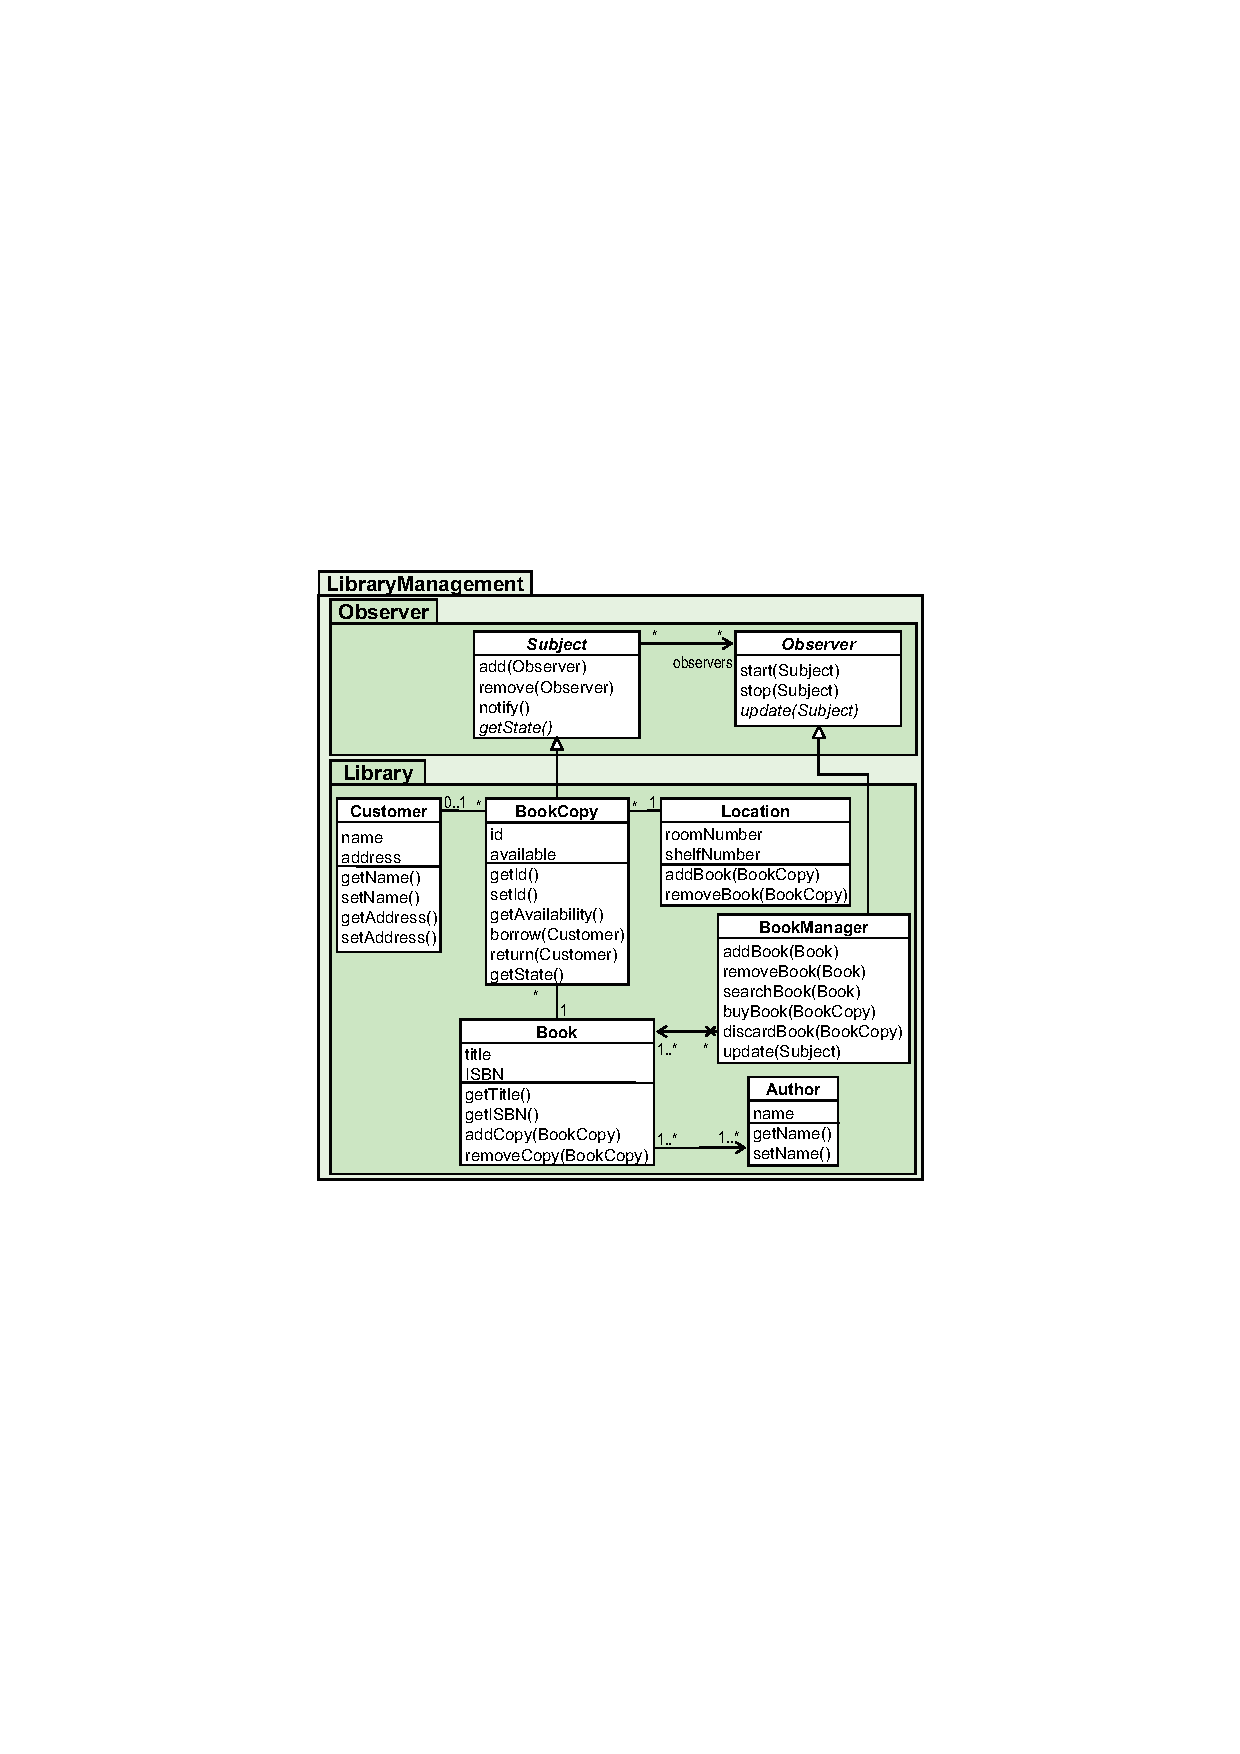
\includegraphics[width=0.7\textwidth]{figures/figure1}
	\caption{Sample figure}
	\label{fig:samplefigure_pdf}
\end{figure}


\section{Fonts}

When introducing important terms for the first time use \emph{emphasize}. For a consistent look and feel of proper names like {\cd} and {\uml{Observer}} pattern you may define macros in the main document \texttt{thesis.tex}.

\section{Code}

For short code fragments use the \textit{verbatim} environment.

\begin{verbatim}
//Start Program
System.out.println("Hello World!");
//End Program
\end{verbatim}

A much better alternative is the \textit{algorithm} environment (cf. Algorithm~\ref{alg:samplealgorithm}). This environment offers special formatting features for loops, operations and comments.

\begin{comment} % my algo package has different syntax
\begin{algorithm}[t]
\SetKwData{Left}{left}
\SetKwData{This}{this}
\SetKwData{Up}{up}
\SetKwFunction{Union}{Union}
\SetKwFunction{FindCompress}{FindCompress}
\SetKwInOut{Input}{input}
\SetKwInOut{Output}{output}

\Input{A bitmap $Im$ of size $w\times l$}
\Output{A partition of the bitmap}

\BlankLine

\emph{special treatment of the first line}\;
\For{$i\leftarrow 2$ \KwTo $l$}{
\emph{special treatment of the first element of line $i$}\;
\For{$j\leftarrow 2$ \KwTo $w$}{\label{forins}
\Left$\leftarrow$ \FindCompress{$Im[i,j-1]$}\;
\Up$\leftarrow$ \FindCompress{$Im[i-1,]$}\;
\This$\leftarrow$ \FindCompress{$Im[i,j]$}\;
\If(\tcp*[r]{O(\Left,\This)==1}){\Left compatible with \This}{\label{lt}
\lIf{\Left $<$ \This}{\Union{\Left,\This}}\;
\lElse{\Union{\This,\Left}\;}
}
\If(\tcp*[r]{O(\Up,\This)==1}){\Up compatible with \This}{\label{ut}
\lIf{\Up $<$ \This}{\Union{\Up,\This}}\;
\tcp{\This is put under \Up to keep tree as flat as possible}\label{cmt}
\lElse{\Union{\This,\Up}}\tcp*[r]{\This linked to \Up}\label{lelse}
}
}
\lForEach{element $e$ of the line $i$}{\FindCompress{p}}
}
\caption{Sample algorithm}\label{alg:samplealgorithm}
\end{algorithm}

\end{comment} 



%%%%%%%%%%%%%%%%%%%%%%%%%%%%%%%%%%%%%%%%%
\chapter{Bibliographic Issues}
\label{ch:bibliographic}
%%%%%%%%%%%%%%%%%%%%%%%%%%%%%%%%%%%%%%%%%

\section{Literature Search}

Information on online libraries and literature search, e.g., interesting magazines, journals, conferences, and organizations may be found at \url{http://www.big.tuwien.ac.at/teaching/info.html}.

\section{BibTeX}

BibTeX should be used for referencing.

The LaTeX source document of this pdf document provides you with different samples for references to journals~\cite{jour:B2BServices}, conference papers~\cite{proc:TheWebMLApproach}, books~\cite{book:umlatwork}, book chapters~\cite{incoll:ErhardKonrad1992}, electronic standards~\cite{man:BPEL}, dissertations~\cite{phdthesis:manuelWimmer}, masters' theses~\cite{mast:AUMLProfile}, and web sites~\cite{misc:BIGWebsite}. The respective BibTeX entries may be found in the file \texttt{references.bib}. For administration of the BibTeX references we recommend \url{http://www.citeulike.org} or JabRef for offline administration, respectively.


%%%%%%%%%%%%%%%%%%%%%%%%%%%%%%%%%%%%%%%%%
%%% BACKMATTER %%%%%%%%%%%%%%%%%%%%%%%%%%
%%%%%%%%%%%%%%%%%%%%%%%%%%%%%%%%%%%%%%%%%

\end{comment}

\chapter{Constructive Proofs}

\section{WT: Interpolation extraction in one pass}

easy for constants, just as in huang but in one pass

terms can grow unpredictably, order cannot be determined during pass

\section{WT: Interpolation extraction in two passes}

\subsection{huang proof revisited}

\subsubsection{propositional part}

Let $\Gamma \cup \Delta$ be unsatisfiable. Let $\pi$ be a proof of $\square$ from $\Gamma \cup \Delta$. Then $\PI$ is a function that returns a interpolant w.r.t. the current clause. 

\begin{defi}
	$\theta$ is a \defiemph{propositional interpolant} with respect to a clause $C$ in a resolution refutation $\pi$ of $\Gamma \cup \Delta$ if 
	\label{def:rel_prop_interpol}
	\begin{compactenum}
		\item $\Gamma \entails \theta \lor C$
			\label{rel_prop_interpol_cond1}
		\item $\Delta \entails \lnot \theta \lor C$
			\label{rel_prop_interpol_cond2}
		\item $\Pred(\theta) \subseteq (\Pred(\Gamma) \intersect \Pred(\Delta)) \cup \{\top, \bot\} $.
			\label{rel_prop_interpol_cond_lang}
			\qedhere
	\end{compactenum}
\end{defi}

The third condition will sometimes be referred to as \emph{language restriction}.
It is easy to see that a propositional interpolant with respect to $\square$ is a propositional interpolant\todo{add this to the definition, i.e.~possible define rel prop interpol from prop interpol}, i.e.~it is an interpolant without the language restriction on constant, variable and function symbols.

We proceed by defining a procedure $\PI$ which extracts interpolants from a resolution refutation.

\begin{defi}
	\defiemph{$\PI$} is defined as follows:
\begin{itemize}
	\item[Base case.]
		If $C \in \Gamma$, $\PI(C) = \bot$. 
		If otherwise $C \in \Delta$, $\Delta(C) = \top$. 
	\item[Resolution.]
	\label{def:PI_resolution}
		Suppose the clause $C$ is the result of a resolution step. Then it has the following form: 

%	\begin{prooftree}
%		\AxiomCm{C_1: D \lor l}
%		\AxiomCm{C_2: E \lor \lnot l'}
%		\RightLabelm{\quad l\sigma = l'\sigma}
%		\BinaryInfCm{C: (D\lor E)\sigma}
%	\end{prooftree}
		%\todo{write as prooftree? (not necessary, but nicer)}
		If the clause $C$ is the result of a resolution step of $C_1: D \lor l$ and $C_2: E \lor \lnot l'$ using a unifier $\sigma$ such that $l\sigma = l'\sigma$, then $\PI(C)$ is defined as follows:
	%$\PI(C)$ is defined according to this case distinction:
		\begin{enumerate}
			\item If $\Pred(l) \in \Lang(\Gamma) \setminus \Lang(\Delta)$:\todo{change to "is $\Gamma$-colored?"} $\PI(C) = [\PI(C_1) \lor \PI(C_2)]\sigma$
			\item If $\Pred(l) \in \Lang(\Delta) \setminus \Lang(\Gamma)$: $\PI(C) = [\PI(C_1) \land \PI(C_2)]\sigma$
			\item If $\Pred(l) \in \Lang(\Gamma) \intersect \Lang(\Delta)$: $\PI(C) = [(l \land \PI(C_2)) \lor (l' \land \PI(C_1)) ]\sigma $
		\end{enumerate}

	\item[Factorisation.]
		If the clause $C$ is the result of a factorisation of $C_1: l \lor l' \lor D$ using a unifier $\sigma$ such that $l\sigma = l'\sigma$, then $\PI(C) = \PI(C_1)\sigma$.

	\item[Paramodulation.]
		If the clause $C$ is the result of a paramodulation of $C_1: s=t \lor C$ and $C_2: D[r]$ using a unifier $\sigma$ such that $r\sigma = s\sigma$, then $\PI(C)$ is defined according to the following case distinction:
		\begin{enumerate}
			\item If $r$ occurs in a maximal $\Delta$-term $h(r)$ in $D[r]$ and $h(r)$ occurs more than once in $D[r] \lor \PI(D[r])$:
				\label{def:PI_paramod_1}
				\newline
				$\PI(C) = [ ( s=t \land \PI(C_2) ) \lor (s\neq t \land \PI(C_1)) ]\sigma \lor (s=t \land h(s) \neq h(t))$ 
			\item If $r$ occurs in a maximal $\Gamma$-term $h(r)$ in $D[r]$ and $h(r)$ occurs more than once in $D[r] \lor \PI(D[r])$:
				\label{def:PI_paramod_2}
				\newline
				$\PI(C) = [ ( s=t \land \PI(C_2) ) \lor (s\neq t \land \PI(C_1)) ]\sigma \land (s\neq t \lor h(s) = h(t))$ 
			\item Otherwise:
				\label{def:PI_paramod_3}
				\newline
				$\PI(C) = [ ( s=t \land \PI(C_2) ) \lor (s\neq t \land \PI(C_1)) ]\sigma$ \qedhere

		\end{enumerate}
\end{itemize}
\end{defi}


\begin{prop}
	Let $C$ be a clause of a resolution refutation.
	Then $\PI(C)$ is a propositional interpolant with respect to $C$. 
\end{prop}
\begin{proof}
	Proof by induction on the number of rule applications including the following strenghtenings:
	$\Gamma \entails \PI(C) \lor C_\Gamma$ and
	$\Delta \entails \lnot \PI(C) \lor C_\Delta$, where $D_\Phi$ denotes the clause D with only the literals which are contained in $\Lang(\Phi)$. They clearly imply conditions \ref{rel_prop_interpol_cond1} and \ref{rel_prop_interpol_cond2} of definition \ref{def:rel_prop_interpol}. 

\begin{itemize}
	\item[Base case.]
	Suppose no rules were applied. We distinguish two possible cases:
	\begin{enumerate}
		\item $C \in \Gamma$.
			Then $\PI(C) = \bot$. Clearly $\Gamma \entails \bot \lor C_\Gamma$ as $C_\Gamma = C \in \Gamma$, $\Delta \entails \lnot \bot \lor C_\Delta$ and $\bot$ satisfies the restriction on the language.

		\item $C \in \Delta$.
			Then $\PI(C) = \top$. Clearly $\Gamma \entails \top \lor C_\Gamma$, $\Delta \entails \lnot \top \lor C_\Delta$ as $C_\Delta = C \in \Delta$ and $\top$ satisfies the restriction on the language.
	\end{enumerate}

	Suppose the property holds for $n$ rule applications.
	We show that it holds for $n+1$ applications by considering the last one:

\item[Resolution.]
	Suppose the last rule application is an instance of resolution. Then it is of the form:
	\begin{prooftree}
		\AxiomCm{C_1: D \lor l}
		\AxiomCm{C_2: E \lor \lnot l'}
		\RightLabelm{\quad l\sigma = l'\sigma}
		\BinaryInfCm{C: (D\lor E)\sigma}
	\end{prooftree}

	By the induction hypothesis, we can assume that:

	$\Gamma \entails \PI(C_1) \lor (D\lor l)_\Gamma$

	$\Delta \entails \lnot \PI(C_1) \lor (D\lor l)_\Delta$

	$\Gamma \entails \PI(C_2) \lor (E\lor \lnot l')_\Gamma$

	$\Delta \entails \lnot \PI(C_2) \lor (E\lor \lnot l')_\Delta$

		We consider the respective cases from definition \ref{def:PI_resolution}:

			\begin{enumerate}
				\item $\Pred(l) \in \Lang(\Gamma) \setminus \Lang(\Delta)$:
					\label{huang_proof_prop_case_1}
					Then $\PI(C) = [\PI(C_1) \lor \PI(C_2)]\sigma$. 

					As $\Pred(l) \in \Lang(\Gamma)$,
					$\Gamma \entails (\PI(C_1) \lor D_\Gamma\lor l)\sigma$
					as well as $\Gamma \entails (\PI(C_2) \lor E_\Gamma\lor \lnot l')\sigma$.
					By a resolution step, we get $\Gamma \entails (\PI(C_1) \lor \PI(C_2))\sigma \lor ((D \lor E)\sigma)_\Gamma$.

					Furthermore, as $\Pred(l) \not\in \Lang(\PI)$, 
					$\Delta \entails (\lnot\PI(C_1) \lor D_\Delta)\sigma$
					as well as $\Delta \entails (\lnot\PI(C_2) \lor E_\Delta)\sigma$.
					Hence it certainly holds that $\Delta \entails (\lnot \PI(C_1) \lor \lnot\PI(C_2))\sigma \lor (D \lor E)\sigma_\Delta$.

					The language restriction clearly remains satisfied as no nonlogical symbols are added.

				\item $\Pred(l) \in \Lang(\Delta) \setminus \Lang(\Gamma)$: 
					\label{huang_proof_prop_case_2}
					Then $\PI(C) = [\PI(C_1) \land \PI(C_2)]\sigma$. 

					As $\Pred(l) \not\in \Lang(\Gamma)$,
					$\Gamma \entails (\PI(C_1) \lor D_\Gamma)\sigma$
					as well as $\Gamma \entails (\PI(C_2) \lor E_\Gamma)\sigma$.
					Suppose that in a model $M$ of $\Gamma$, $M \cancel \entails D_\Gamma$ and $M \cancel \entails E_\Gamma$. Then $M \entails \PI(C_1) \land \PI(C_2)$.
					Hence 
					$\Gamma \entails (\PI(C_1) \land \PI(C_2))\sigma \lor ((D \lor E)\sigma)_\Gamma$.

					Furthermore due to $\Pred(l) \in \Lang(\Delta)$,
					$\Delta \entails (\lnot\PI(C_1) \lor D_\Delta \lor l)\sigma$
					as well as $\Delta \entails (\lnot\PI(C_2) \lor E_\Delta \lor \lnot l')\sigma$.
					By a resolution step, we get $\Delta \entails (\lnot\PI(C_1) \lor \lnot\PI(C_2))\sigma \lor (D_\Delta \lor E_\Delta)\sigma $
					and hence 
					$\Delta \entails \lnot (\PI(C_1) \land \PI(C_2))\sigma \lor (D_\Delta \lor E_\Delta)\sigma $.

					The language restriction again remains intact.

				\item $\Pred(l) \in \Lang(\Delta) \intersect \Lang(\Gamma)$:
					Then $\PI(C) = [(l \land \PI(C_2)) \lor (\lnot l' \land \PI(C_1)) ]\sigma $

					First, we have to show that 
					$ \Gamma \entails [(l \land \PI(C_2)) \lor (l' \land \PI(C_1)) ]\sigma \lor ((D \lor E)\sigma)_\Gamma$.
					Suppose that in a model $M$ of $\Gamma$, $M \cancel \entails D_\Gamma$ and $\Gamma \cancel \entails E$. Otherwise we are done.
					The induction assumtion hence simplifies to $M \entails \PI(C_1) \lor l$ and $M \entails \PI(C_2) \lor \lnot l'$ respectively.
					As $l\sigma = l'\sigma$, by a case distinction argument on the truth value of $l\sigma$, we get that either $M \entails (l \land \PI(C_2))\sigma$ or $M \entails  (\lnot l' \land \PI(C_1))\sigma$.


					Second, we show that 
					$\Delta \entails ((l \lor \lnot \PI(C_1)) \land (\lnot l' \lor \lnot \PI(C_2)))\sigma \lor ((D \lor E)\sigma)_\Delta$.
					Suppose again that in a model $M$ of $\Delta$, $M \cancel \entails D_\Delta$ and $\Gamma \cancel \entails E_\Delta$. 
					Then the required statement follows from the induction hypothesis.
					
					The language condition remains satisfied as only the common literal $l$ is added to the interpolant.


			\end{enumerate}

		\item[Factorisation.]	
			Suppose the last rule application is an instance of factorisation. Then it is of the form:
			\begin{prooftree}
				\AxiomCm{C_1: l \lor l' \lor D}
				\RightLabelm{\quad \sigma = \mgu(l, l')}
				\UnaryInfCm{C_1: (l \lor D)\sigma}
			\end{prooftree}

			Then the propositional interpolant $\PI(C)$ is defined as $\PI(C_1)$.
			By the induction hypothesis, we have:

			$\Gamma \entails \PI(C_1) \lor (l \lor l' \lor D)_\Gamma$

			$\Delta \entails \PI(C_1) \lor (l \lor l' \lor D)_\Delta$

			It is easy to see that then also:

			$\Gamma \entails (\PI(C_1)\lor (l \lor D)_\Gamma)\sigma$

			$\Delta \entails (\PI(C_1)\sigma \lor (l \lor D)_\Delta)\sigma$

			The restriction on the language trivially remains intract.
			

		\item[Paramodulation.]	
			Suppose the last rule application is an instance of paramodulation. Then it is of the form:
			\begin{prooftree}
				\AxiomCm{C_1: D \lor s=t}
				\AxiomCm{C_2: E[r]}
				\RightLabel{$\quad \sigma = \mgu(s, r)$}
				\BinaryInfCm{C: (D \lor E[t])\sigma}
			\end{prooftree}

			By the induction hypothesis, we have:

			$\Gamma \entails \PI(C_1) \lor (D\lor s=t)_\Gamma$

			$\Delta \entails \lnot \PI(C_1) \lor (D\lor s=t)_\Delta$

			$\Gamma \entails \PI(C_2) \lor (E[r])_\Gamma$

			$\Delta \entails \lnot \PI(C_2) \lor (E[r])_\Delta$

			First, we show that $\PI(C)$ as constructed in case \ref{def:PI_paramod_3} of the definition is a propositional interpolant in any of these cases:

			$\PI(C) = (s=t \land \PI(C_2)) \lor (s\neq t \land \PI(C_1)) $
			
			Suppose that in a model $M$ of $\Gamma$, $M \cancel \entails D\sigma$ and $M \cancel \entails E[t]\sigma$. Otherwise we are done.
			Furthermore, assume that $M \entails (s=t)\sigma$. Then $M \cancel \entails E[r]\sigma$, but then necessarily $M \entails \PI(C_2)\sigma$. \\
			On the other hand, suppose $M \entails (s\neq t)\sigma$. As also $M \cancel \entails D\sigma$, $M \entails \PI(C_1)\sigma$.
			Consequently, $M \entails [(s=t \land \PI(C_2)) \lor (s\neq t \land \PI(C_1))]\sigma \lor [(D \lor E)_\Gamma]\sigma$

			By an analogous argument, we get $\Delta \entails [(s=t \land \lnot \PI(C_2)) \lor (s\neq t \land \lnot \PI(C_1))]\sigma \lor [(D \lor E)_\Delta]\sigma$,
			which implies
			$\Delta \entails [( s\neq t \lor \lnot \PI(C_2)) \land (s = t \lor \lnot \PI(C_1))]\sigma \lor ((D \lor E)_\Delta)\sigma $

			%By a similar case distinction for a model $M$ of $\Delta$ and assuming that $M \cancel \entails D_\Delta$ and $M \cancel \entails E_\Delta$, we get that if $M \entails (s=t)\sigma$, $M \entails \lnot P$, which implies

			The language restriction again remains satisfied as the only predicate, that is added to the interpolant, is $=$.

			This concludes the argumentation for case \ref{def:PI_paramod_3}. 

			The interpolant of case \ref{def:PI_paramod_1} differs only by an additional formula added via a disjunction and hence condition \ref{rel_prop_interpol_cond1} of definition \ref{def:rel_prop_interpol} holds by the above reasoning.
			As the adjoined formula is a contradiction, its negation is valid which in combination with the above reasoning establishes condition \ref{rel_prop_interpol_cond2}.
			Since no new predicated are added, the language condition remains intact. 

			The situation in case \ref{def:PI_paramod_2} is somewhat symmetric: 
			As a tautology is added to the interpolant with respect to case \ref{def:PI_paramod_1}, condition \ref{rel_prop_interpol_cond1} is satisfied by the above reasoning.
			For condition \ref{rel_prop_interpol_cond2}, consider that the negated interpolant of case \ref{def:PI_paramod_1} implies the negated interpolant of this case.
			The language condition again remains intact.
			\qedhere
	\end{itemize}

	proof that we are allowed to overbind

	TODO: define procedure

	TODO: proof

	\end{proof}


	\subsubsection{overbinding}

	Algorithm (input: propositional interpolant $\theta$):
	\begin{enumerate}
		\item Let $t_1, \ldots, t_n$ be the maximal occurrences of noncommon terms in $\theta$. Order $t_i$ ascendingly by term size. 
		\item Let $\theta^*$ be $\theta$ with maximal occurrences of $\Delta$-terms $r_1, \ldots, r_k$ replaced by fresh variables $x_1, \ldots, x_k$ and maximal occurrences of $\Gamma$-terms $s_1, \ldots, s_{n-k}$ by fresh variables $x_{k+1}, \ldots, x_{n}$
		\item Return $Q_1 x_1, \ldots Q_n x_n \theta^*$, where $Q_i$ is $\forall$ if $t_i$ is a $\Delta$-term and $\exists$ otherwise.
	\end{enumerate}

	Language condition easily established. To prove:

	$\Gamma \entails Q_1 x_1, \ldots Q_n x_n \theta^*$

	$\Delta \entails \lnot Q_1 x_1, \ldots Q_n x_n \theta^*$

	We know that $\theta$ works, just the terms are missing.

	\clearpage
	\section{Attempt without $P_P$}:


	\begin{defi}
		\label{def:overline}
		Overline as in paper, replace $\Delta$-terms $t_1, \ldots, t_k$ by respective fresh variables in parenthesis
	\end{defi}

	\begin{lemma}
		\label{lemma:overline}
		$(\overline{C\sigma}(x_1, \ldots, x_n))$ reduces to
		$(\overline{C}(x_1, \ldots, x_n))\sigma'$, where $\sigma' = \sigma[t_1 / x_1]\ldots[t_n / x_n]$.

		$(\overline{C}(x_1, \ldots, x_n))\sigma$ reduces to
		$(\overline{C\sigma'}(x_1, \ldots, x_n))$ if $\sigma$ does not change any of $x_1, \ldots, x_n$ or any of $t_1, \ldots, t_n$.\qedhere

		\todo[inline]{it would work to fix substitutions of $x_i$ by substituting $t_i$ for that instead, as long as the result isn't another $t_i$, but this isn't actually relevant here.}
		
	\end{lemma}

	\begin{prop}
		$\Gamma = \overline{\Gamma}(x_1, \ldots, x_n)$.
	\end{prop}
	\begin{proof}
		By definition, $\Delta$-terms only appear in $\Delta$ and not in $\Gamma$. 
	\end{proof}

	\begin{lemma} $ \Gamma \entails \overline{(\PI(C) \lor C)}(x_1, \ldots, x_n) $.
		\label{lemma:gamma_entails_interpolant}
	\end{lemma}

	\begin{proof}
	By induction on the resultion refutation.

	Base case:
	Either $C \in \Gamma$, then it does not contain $\Delta$-terms.
	Otherwise $C \in \Delta$ and $\PI(C) = \top$.

	Induction step:
	\begin{description}
		\item{Resolution.}
			\begin{prooftree}
				\AxiomCm{C_1: D \lor l}
				\AxiomCm{C_2: E \lor \lnot l'}
				\RightLabelm{\quad l\sigma = l'\sigma}
				\BinaryInfCm{C: (D\lor E)\sigma}
			\end{prooftree}

			By the induction hypothesis, we can assume that:

			$\Gamma \entails \overline{\PI(C_1) \lor (D\lor l)}(x_1, \ldots, x_n)$

			$\Gamma \entails \overline{\PI(C_2) \lor (E\lor \lnot l')}(x_{1}, \ldots, x_n)$

			\begin{enumerate}
				\item $\Pred(l) \in \Lang(\Gamma) \setminus \Lang(\Delta)$:
					Then $\PI(C) = [\PI(C_1) \lor \PI(C_2)]\sigma$. 

					We show that $\Gamma \entails \overline{(\PI(C_1) \lor \PI(C_2) \lor D \lor E)\sigma}(x_1, \ldots, x_n) $.
					This is by lemma \ref{lemma:overline} with $\sigma'$ as in the lemma equivalent to
					$\Gamma \entails \overline{(\PI(C_1) \lor \PI(C_2) \lor D \lor E)}(x_1, \ldots, x_n)\sigma' $.

					By Lemma 11 (Huang) and the induction hypothesis,

					$\Gamma \entails \overline{\PI(C_1)} \lor \overline{D} \lor \overline l$

					$\Gamma \entails \overline{\PI(C_2)} \lor \overline{E} \lor \overline{\lnot l'}$

					As $l\sigma = l'\sigma$, $\overline{l\sigma} = \overline{l'\sigma}$.

					Hence $\Gamma \entails \overline{\PI(C_1)} \lor \overline{D} \lor \overline{\PI(C_2)} \lor \overline{E}$
					and again by Lemma 11 (Huang), 
					$\Gamma \entails \overline{\PI(C_1) \lor D \lor \PI(C_2) \lor E}$.

					Also
					$\Gamma \entails \overline{\PI(C_1) \lor D \lor \PI(C_2) \lor E}\sigma$.
					As $ t_1, \ldots, t_n $ do not appear in $\overline{\PI(C_1) \lor D \lor \PI(C_2) \lor E}$ and these are the only variables where $\sigma$ and $\sigma'$ differs, we get that 
					$\Gamma \entails \overline{\PI(C_1) \lor D \lor \PI(C_2) \lor E}\sigma'$.


				\item $\Pred(l) \in \Lang(\Delta) \setminus \Lang(\Gamma)$:
					Then $\PI(C) = [\PI(C_1) \land \PI(C_2)]\sigma$. 

					We show that $\Gamma \entails \overline{((\PI(C_1) \land \PI(C_2)) \lor D \lor E)\sigma}(x_1, \ldots, x_n) $.
					By lemma \ref{lemma:overline} with $\sigma'$ as in the lemma,
					$\Gamma \entails \overline{((\PI(C_1) \land \PI(C_2)) \lor D \lor E)}(x_1, \ldots, x_n) \sigma'$.

					TODO


			\end{enumerate}

		\item{Paramodulation.}

			\begin{prooftree}
				\AxiomCm{C_1: D \lor s=t}
				\AxiomCm{C_2: E[r]}
				\RightLabel{$\quad \sigma = \mgu(s, r)$}
				\BinaryInfCm{C: (D \lor E[t])\sigma}
			\end{prooftree}

			By the induction hypothesis, we have:

			$\Gamma \entails \overline{\PI(C_1) \lor (D\lor s=t)}$

			$\Gamma \entails \overline{\PI(C_2) \lor (E[r])}$



	easy case:
			$\PI(C) = [ ( s=t \land \PI(C_2) ) \lor (s\neq t \land \PI(C_1)) ]\sigma$

			to show:
			$\Gamma \entails \overline{ [ (( s=t \land \PI(C_2) ) \lor (s\neq t \land \PI(C_1))) \lor (D \lor E[t]) ]\sigma} $

			proof idea: either $s=t$, then also $\PI(C_2)$, or else $s\neq t$, but then also $\PI(C_1)$

			by lemma \ref{lemma:overline} for $\sigma'$ as in lemma, 
			$\Gamma \entails \overline{ (( s=t \land \PI(C_2) ) \lor (s\neq t \land \PI(C_1))) \lor (D \lor E[t]) }\sigma' $

			by lemma 11 (huang)
			$\Gamma \entails [((\overline{s}=\overline{t} \land \overline{\PI(C_2)} ) \lor (\overline{s\neq t} \land \overline{\PI(C_1)})) \lor (\overline{D} \lor \overline{E[t]}) ]\sigma' $

			reformulate:
			$\Gamma \entails ((\overline{s}\sigma'=\overline{t}\sigma' \land \overline{\PI(C_2)}\sigma' ) \lor (\overline{s}\sigma'\neq \overline{t}\sigma' \land \overline{\PI(C_1)}\sigma')) \lor (\overline{D}\sigma' \lor \overline{E[t]}\sigma') $

			By the rule: $s\sigma = r\sigma$, hence also $\overline{s\sigma} = \overline{r\sigma}$ and $\overline{s}\sigma' = \overline{r}\sigma'$ REALLY TRUE? -- think so\dots

			Suppose $M \entails \Gamma$ and $M \not \entails (\overline{D}\sigma' \lor \overline{E[t]}\sigma') $.

			Suppose $M \entails \overline{s}\sigma' = \overline{t}\sigma'$.

			By induction hypothesis (and lemma 11 (huang) and adding the substitution $\sigma'$), 
			$\Gamma \entails \overline{\PI(C_2)}\sigma' \lor \overline{(E[r])}\sigma'$.

		However by assumption $\Gamma \not \entails \overline{E[t]}\sigma'$.

		Hence $\Gamma \not \entails \overline{E[s]}\sigma'$, and
		$\Gamma \not \entails \overline{E[r]}\sigma'$. Therefore $\Gamma \entails \overline{\PI(C_2)}\sigma'$.


		Suppose on the other hand $M \entails \overline{s}\sigma' \neq \overline{t}\sigma'$.

		By the induction hypothesis, 
		$M \entails \overline{\PI(C_1)}\sigma' \lor (\overline{D}\sigma'\lor (\overline{s}=\overline{t})\sigma')$,
		hence then $M \entails \overline{\PI(C_1)}\sigma'$.

		Consequently, 
		$M \entails (\overline{s}\sigma' \neq \overline{t}\sigma' \land \overline{\PI(C_1)}\sigma') \lor (\overline{s}\sigma' = \overline{t}\sigma' \land \overline{\PI(C_2)}\sigma')$.

		By lemma 11 (huang), 
		$M \entails \overline{(s \neq {t} \land {\PI(C_1)} \lor ({s} = {t} \land \PI(C_2))}\sigma'$.

		Hence 
		$\Gamma \entails \overline{(s \neq {t} \land {\PI(C_1)} \lor ({s} = {t} \land \PI(C_2))}\sigma' \lor (\overline{D} \lor \overline{E[t]})\sigma') $.

		IS THIS REALLY WHAT I NEED TO SHOW?


\end{description}
\end{proof}



\subsection{final step of huang's proof}

\begin{thm}
	$Q_1 z_1 \ldots Q_n z_n \PI(\square)^*(z_1, \ldots, z_n)$ is a craig interpolant (order as in huang).
\end{thm}
\begin{proof}
	By lemma \ref{lemma:gamma_entails_interpolant}, $\Gamma \entails \forall x_1 \ldots \forall x_n \overline{\PI(\square)}(x_1, \ldots, x_n)$.

	The terms in $\overline{PI(\square)}$ are either among the $x_i$, $1 \leq i \leq n$ or grey terms or $\Gamma$-terms.
	Let $t$ be a maximal $\Gamma$-term in $\overline{\PI(\square)}$.
	Then it is of the form $f(x_{i_1}, \ldots, x_{i_{n_x}}, u_1, \ldots, u_{n_u}, v_1, \ldots, v_{n_v})$, where $f$ is $\Gamma$-colored, the $x_j$ are as before, the $u_j$ are grey terms and the $v_j$ are $\Gamma$-terms.\todo{basically only need the $x_j$}{}
	Note that the $\Delta$-terms, which are replaced by the $x_{i_1}, \ldots, x_{i_{n_x}}$ are of strictly smaller size than $t$ as they are ``strict'' subterms of $t$.

	In $\PI(\square)^*$, $t$ will be replaced by some $z_j$, which is existentially quantified.
	For this $z_j$, $t$ is a witness as due to the quantifier ordering, all the $x_{i_1}, \ldots, x_{i_{n_x}}$ will be quantified before the existential quantification of $z_j$.
	Therefore $\Gamma \entails Q_1 z_1 \ldots Q_n z_n \PI(\square)^*(z_1, \ldots, z_n)$

\end{proof}





\chapter{Notes}


\newcommand{\seq}{\vdash} % the sequent sign
\newcommand{\impl}{\supset} %logical connectives: implies, not, and, or
\renewcommand{\lnot}{\neg}
\renewcommand{\land}{\wedge}
\renewcommand{\lor}{\vee}


\subsubsection*{Axioms}

\begin{prooftree}
\AxiomCm{}
\RightLabelm{(\mt{Identity Axiom})}
\UnaryInfCm{\Gamma, A \seq \Delta, A}
\end{prooftree}
Interpolant: $A$

\begin{prooftree}
\AxiomCm{}
\RightLabelm{(\mt{Reflexivity Axiom})}
\UnaryInfCm{\Gamma \seq \Delta, t = t}
\end{prooftree}
Interpolant: $\top$

\subsubsection*{Cut}

  \begin{prooftree}
  \AxiomCm{\Gamma \seq \Delta, A}
  \AxiomCm{\Sigma, A \seq \Pi}
  \RightLabelm{(\mt{cut})}
  \BinaryInfCm{\Gamma, \Sigma \seq \Delta, \Pi}
  \end{prooftree}
Interpolant: TODO

\subsubsection*{Structural rules}

EASY

\begin{multicols}{2}

  \subsubsection*{Left rules}

  \begin{prooftree}
  \AxiomCm{\Gamma \seq \Delta}
  \RightLabelm{(\mt{w:l})}
  \UnaryInfCm{\Gamma, A \seq \Delta}
  \end{prooftree}

  \begin{prooftree}
  \AxiomCm{\Gamma, A, A \seq \Delta}
  \RightLabelm{(\mt{c:l})}
  \UnaryInfCm{\Gamma, A \seq \Delta}
  \end{prooftree}

  \subsubsection*{Right rules}

  \begin{prooftree}
  \AxiomCm{\Gamma \seq \Delta}
  \RightLabelm{(\mt{w:r})}
  \UnaryInfCm{\Gamma \seq \Delta, A}
  \end{prooftree}

  \begin{prooftree}
  \AxiomCm{\Gamma \seq \Delta, A, A}
  \RightLabelm{(\mt{c:r})}
  \UnaryInfCm{\Gamma \seq \Delta, A}
  \end{prooftree}

\end{multicols}



\subsubsection*{Propositional rules}

\begin{multicols}{2}

  \subsubsection*{Left rules}

  \begin{prooftree}
  \AxiomCm{\Gamma, A \seq \Delta}
  \RightLabelm{(\land\mt{l}_1)}
  \UnaryInfCm{\Gamma, A \land B \seq \Delta}
  \end{prooftree}
Interpolant: $I_1$

  \begin{prooftree}
  \AxiomCm{\Gamma, B \seq \Delta}
  \RightLabelm{(\land\mt{l}_2)}
  \UnaryInfCm{\Gamma, A \land B \seq \Delta}
  \end{prooftree}
Interpolant: $I_1$

  \begin{prooftree}
  \AxiomCm{\Gamma, A \seq \Delta}
  \AxiomCm{\Sigma, B \seq \Pi}
  \RightLabelm{(\lor\mt{:l})}
  \BinaryInfCm{\Gamma, \Sigma, A \lor B \seq \Delta, \Pi}
  \end{prooftree}
Interpolant: $I_1 \lor I_2$

  \begin{prooftree}
  \AxiomCm{\Gamma \seq \Delta, A}
  \RightLabelm{(\lnot\mt{:l})}
  \UnaryInfCm{\Gamma, \neg A \seq \Delta}
  \end{prooftree}
Interpolant: $I_1$ (considering proper coloring (global view))

  \begin{prooftree}
  \AxiomCm{\Gamma \seq \Delta, A}
  \AxiomCm{\Sigma, B \seq \Pi}
  \RightLabelm{(\impl\mt{:l})}
  \BinaryInfCm{\Gamma, \Sigma, A \impl B \seq \Delta, \Pi}
  \end{prooftree}
Interpolant: $I_1 \lor I_2$ (again with global view)



  \subsubsection*{Right rules}

  \begin{prooftree}
  \AxiomCm{\Gamma \seq \Delta, A}
  \AxiomCm{\Sigma \seq \Pi, B}
  \RightLabelm{(\land\mt{:r})}
  \BinaryInfCm{\Gamma, \Sigma \seq \Delta, \Pi, A \land B}
  \end{prooftree}
Interpolant: $I_1 \land I_2$

  \begin{prooftree}
  \AxiomCm{\Gamma \seq \Delta, A}
  \RightLabelm{(\lor\mt{:r}_1)}
  \UnaryInfCm{\Gamma \seq \Delta, A \lor B}
  \end{prooftree}
Interpolant: $I_1$

  \begin{prooftree}
  \AxiomCm{\Gamma \seq \Delta, B}
  \RightLabelm{(\lor\mt{:r}_2)}
  \UnaryInfCm{\Gamma \seq \Delta, A \lor B}
  \end{prooftree}
Interpolant: $I_1$

  \begin{prooftree}
  \AxiomCm{\Gamma, A\seq \Delta}
  \RightLabelm{(\lnot\mt{:r})}
  \UnaryInfCm{\Gamma \seq \Delta, \neg A}
  \end{prooftree}
Interpolant: $I_1$

  \begin{prooftree}
  \AxiomCm{\Gamma, A \seq B, \Delta}
  \RightLabelm{(\impl\mt{:r})}
  \UnaryInfCm{\Gamma \seq A \impl B, \Delta}
  \end{prooftree}
Interpolant: $I_1 (global view)$

\end{multicols}

\subsubsection*{Quantification roles}

\begin{multicols}{2}

  \subsubsection*{Left rules}

  \begin{prooftree}
  \AxiomCm{\Gamma, A[t/x] \seq \Delta}
  \RightLabelm{(\forall\mt{:l})}
  \UnaryInfCm{\Gamma, \forall x A \seq \Delta}
  \end{prooftree}
Interpolant: $I_1$

  \begin{prooftree}
  \AxiomCm{\Gamma, A[y/x] \seq \Delta}
  \RightLabelm{(\exists\mt{:l})}
  \UnaryInfCm{\Gamma, \exists x A \seq \Delta}
  \end{prooftree}
Interpolant: $I_1$, possibly overbinding eigenvar

  \subsubsection*{Right rules}

  \begin{prooftree}
  \AxiomCm{\Gamma \seq A[y/x] \Delta}
  \RightLabelm{(\forall\mt{:r})}
  \UnaryInfCm{\Gamma \seq \forall x A, \Delta}
  \end{prooftree}
Interpolant: $I_1$, possibly overbinding eigenvar

  \begin{prooftree}
  \AxiomCm{\Gamma \seq A[t/x] \Delta}
  \RightLabelm{(\exists\mt{:r})}
  \UnaryInfCm{\Gamma \seq \exists x A, \Delta}
  \end{prooftree}
Interpolant: $I_1$

\end{multicols}

The variable $y$ must not occur free in $\Gamma$ or $\Delta$. The term $t$ must avoid variable capture, i.e. it must not contain free occurrences of variables bound in $A$.


\subsubsection*{Equational rules}

\begin{multicols}{2}

  \subsubsection*{Left rules}

  \begin{prooftree}
  \AxiomCm{\Gamma \seq \Delta, s=t}
  \AxiomCm{\Sigma, A[T/s] \seq \Pi}
  \RightLabelm{(\mt{=:l}_1)}
  \BinaryInfCm{\Gamma, \Sigma, A[T/t] \seq \Delta, \Pi}
  \end{prooftree}
Interpolant: $I = I_12$.
Proof of first implication:
Supp $M \models LHS$. Then $M \models I_1$

Proof of 2nd implication:
Supp $M \models I$.
As $M \models I_1$, $M \models \Delta \lor s=t$. If $M \models \Delta$, we are done. Otw $M \models s=t$. 

  \begin{prooftree}
  \AxiomCm{\Gamma \seq \Delta, s=t}
  \AxiomCm{\Sigma, A[T/t] \seq \Pi}
  \RightLabelm{(\mt{=:l}_2)}
  \BinaryInfCm{\Gamma, \Sigma, A[T/s] \seq \Delta, \Pi}
  \end{prooftree}
	symmetric

  \subsubsection*{Right rules}

  \begin{prooftree}
  \AxiomCm{\Gamma \seq \Delta, s=t}
  \AxiomCm{\Sigma \seq \Pi, A[T/s]}
  \RightLabelm{(\mt{=:r}_1)}
  \BinaryInfCm{\Gamma, \Sigma \seq \Delta, \Pi, A[T/t]}
  \end{prooftree}
Interpolant: $I = I_1 \land I_2$.
Proof of 2nd implications:
Supp $M \models I$. If $M \models \Pi$, we are done. Otherwise $M \models A[T/s]$. 
If $M \models \Delta$, we are done. Otherwise $M \models s=t$. But then $M \models A[T/t]$.

  \begin{prooftree}
  \AxiomCm{\Gamma \seq \Delta, s=t}
  \AxiomCm{\Sigma, \seq \Pi, A[T/t]}
  \RightLabelm{(\mt{=:r}_2)}
  \BinaryInfCm{\Gamma, \Sigma \seq \Delta, \Pi, A[T/s]}
  \end{prooftree}
	symmetric

\end{multicols}





\appendix

\bibliographystyle{plain}
\bibliography{references}

\end{document}
